\documentclass[main.tex]{subfiles}

\begin{document}
\section{Grafici aggiuntivi}
\begin{figure}[H]
	\centering
	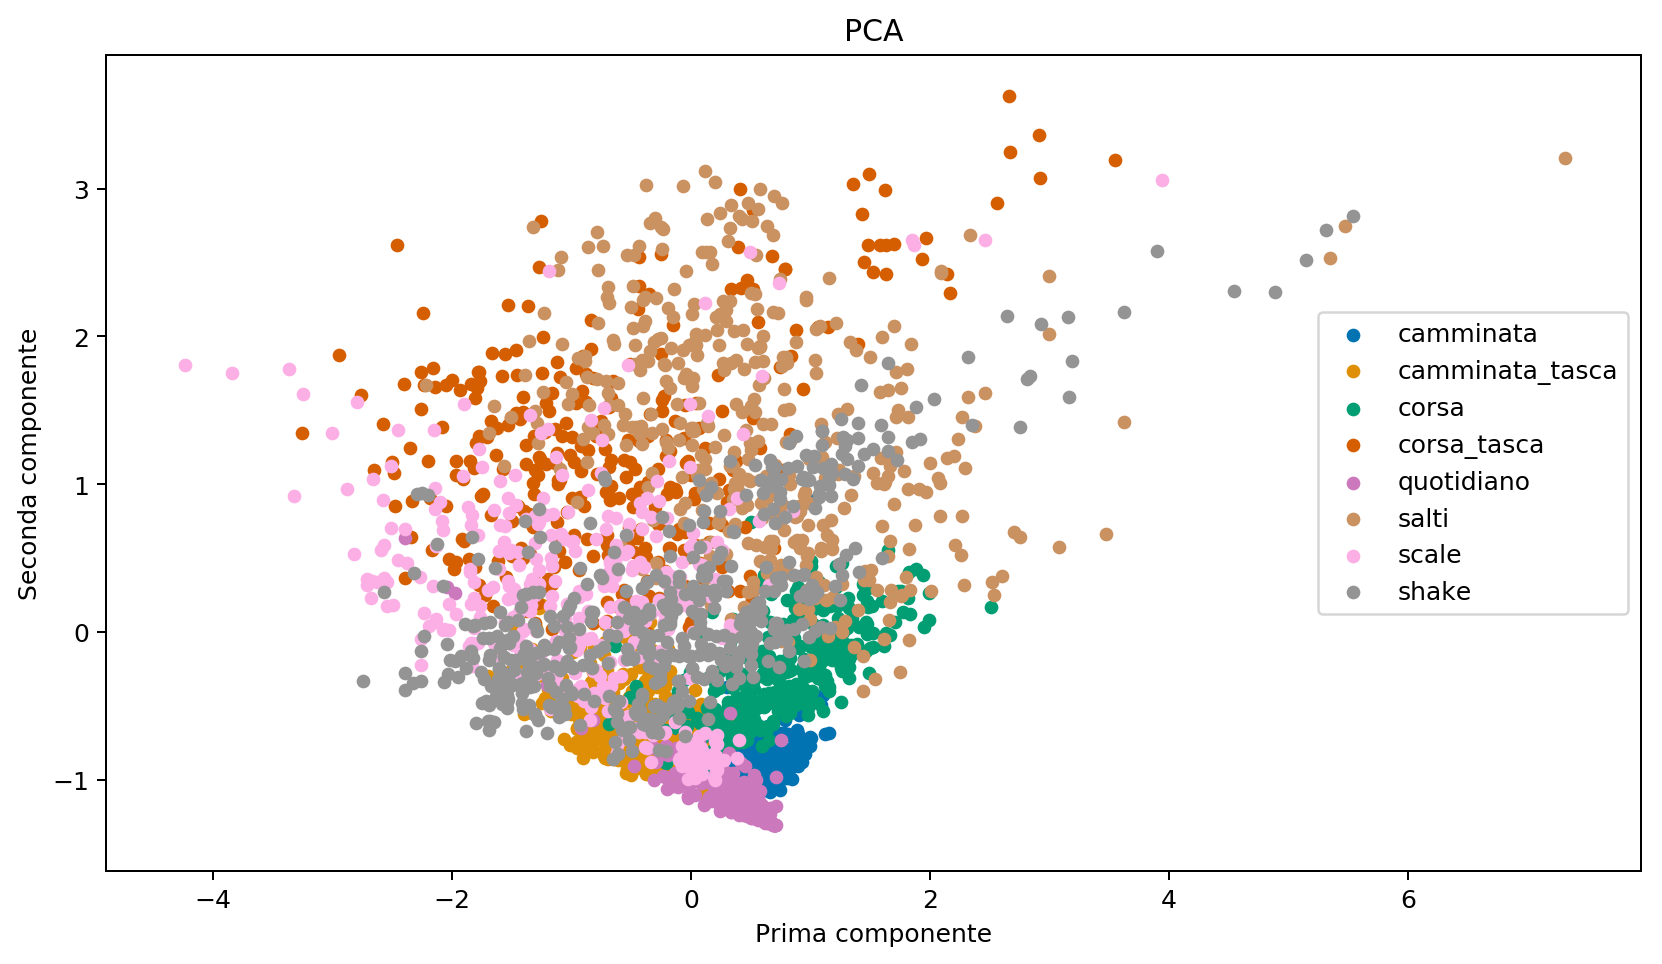
\includegraphics[width=.8\textwidth, keepaspectratio]{../../figure/PCA.png}
	\caption{{ Prime due componenti principali per i dati sbiancati}}
	\label{PCA}
\end{figure}

\foreach\x in {maxA,meanA, medA, minA, MVDeriv}{%
  \begin{figure}[H]
  \centering
    \includegraphics[width=0.8\textwidth]{../../figure/\x}
    \caption{Densità marginali per la variabile \x .}
  \end{figure}
}
\end{document}